\documentclass{llncs}

%\usepackage{amsmath}
%\usepackage[psamsfonts]{amssymb}
\usepackage{url}
\usepackage{xspace}
%\usepackage{authordate1-4}
%\usepackage{makeidx}


% Per includere immagini postscript e bmp:
\usepackage[dvips]{graphicx}
%
\usepackage{ifthen}

\makeatletter
\DeclareRobustCommand\onedot{\futurelet\@let@token\@onedot}
\def\@onedot{\ifx\@let@token.\else.\null\fi\xspace}

\def\eg{\emph{e.g}\onedot} \def\Eg{\emph{E.g}\onedot}
\def\ie{\emph{i.e}\onedot} \def\Ie{\emph{I.e}\onedot}
\def\cf{\emph{c.f}\onedot} \def\Cf{\emph{C.f}\onedot}
\def\etc{\emph{etc}\onedot} \def\vs{\emph{vs}\onedot} 
\def\wrt{w.r.t\onedot} \def\dof{d.o.f\onedot}
\def\etal{\emph{et al}\onedot}
\makeatother

%\interfootnotelinepenalty=10000



%%%%%%%%%%%%%%%%%%%%%%% INIZIO %%%%%%%%%%%%%%%%%%%%%%%
\begin{document}

\mainmatter

\title{Non lo so ancora\thanks{This work was supported by EU project RobotCub (IST-
2004-004370) and CONTACT (NEST-5010).}}

\author{Francesco Orabona\inst{1} \and Giorgio Metta\inst{1,2} \and Giulio Sandini\inst{2}}

\institute{University of Genoa, DIST, Genoa 16145, Italy
\and Italian Institute of Technology, Genoa 16163, Italy}

\maketitle

\begin{abstract}
One of the first
steps of any visual system is that of
locating suitable interest points, `salient regions', in
the scene, to detect events, and eventually to direct
gaze toward these locations. In the last few years,
object-based visual attention models have received an
increasing interest in the literature, the problem, in
this case, being that of creating a model of
`objecthood' that eventually guides a saliency
mechanism. We present here an object-based model of
visual attention and show its instantiation on a
humanoid robot. The robot employs action to learn
and define its own concept of objecthood.
\end{abstract}

\section{Visual Attention\label{attention}}

Spatial attention is often considered as a sort of `filter'
of the incoming information, as a `spotlight',
an internal eye or a sort of `zoom lens'. In particular attention is
believed to be deployed as a spatial gradient, centered on a particular location.
%The experiments of Posner \etal \cite{PosnerSD80} and Downing and Pinker
%\cite{DowningP85} suggest that
%attention is deployed as a spatial gradient, centered on
%a particular location.
Even if supported by numerous findings, maybe this view does not
stress enough the \emph{aim} of the attentional system in an agent with a body.

The external world is sensed
continuously instead of maintaining and updating some
complicated internal model.
This idea has been summarized by O'Regan as:
``The world as an outside memory'' \cite{ORegan92}.
The sentence remarks the fact that it is important
to consider the problem of vision, and perception in general,
deeply rooted in the physical world. Given that, for example,
changes in the world seem to be easily detectable, it
is cheaper to store in memory a rough representation of
the external world, directly accessing to it when a
detailed information is needed and to keep track of the changes.
Moreover, it has no sense to talk about perception without
talking about action, so it is logical to
think that our perception is biased versus a representation
that is useful to act on physical objects.
In the case of visual attention this corresponds to ask
if the attention is deployed on objects (`object-based') or
on space locations (`space-based').
This idea is supported by the discovery in monkeys of a
class of neurons (\emph{mirror neurons}) which not only
fire when the animal performs an action directed to an
object, but also when it sees another monkey or human performing the
same action on the same object \cite{FadigaFGR00}.
Indeed, this tight coupling of perception and action is present in
in visual attention too. In fact, it has been shown in \cite{FischerH04}
that more object-based attention is present during a grasping action, than
space-based one.

%On the other hand there is a recent literature on the
%object-based visual attention, that represents
%the result of a fertile new cross-talk between two
%traditionally separate research fields, one concerning
%visual segmentation and grouping processes, and the
%other concerning selective attention.

Object-based attention theories
argue that attention is directed to an object or a group
of objects, to process specific properties of the selection,
rather than regions of space. There is a
growing evidence both from behavioral and from
neurophysiological studies that shows, in fact, that
selective attention frequently operates on an object based
representational medium in which the
boundaries of segmented objects, and not just spatial
position, determine what is selected and how attention
is deployed (see \cite{Scholl01} for a review). This reflects the fact
that the visual system is optimized for segmenting
complex scenes into representations of objects to be used both for recognition and
action, since perceivers must \emph{interact} with objects and
not just with disembodied spatial locations.

But how can we attend to objects before they are recognized?
To solve this contradiction Rensink \cite{RensinkORC97,Rensink00a}
introduced the notion of `proto-objects', that are volatile units
of visual information that can be bound into a coherent and
stable object when accessed by focused attention and
subsequently validated as actual objects.
In fact, it is generally assumed that the task of grouping pixels
into regions is performed before selective attention is involved
by perceptual organization and Gestalt grouping principles \cite{PalmerR94}.

Guided by these considerations we propose a general proto-object based
visual attention model and we also propose a biological motivated
method to make the system learn the how to pre-segment the images
in proto-objects.


%For example, attention to one part of an object confers
%an attentional advantage to other parts of that object
%\cite{EglyDR94}. Similarly, attention to one aspect of an
%object (\eg its shape) enhances the cortical response to
%other aspects of that object (\eg its color or motion);
%thus, all the attributes of an attended object seem to
%be bound together into a single entity. This concept
%holds even when the attended and ignored objects are
%spatially superimposed.
%O'Craven \etal \cite{OCravenDK99}
%have observed the effects of object-based attention using
%fMRI. In this study, observers looked at a display containing
%a sequence of semitransparent images of
%spatially superimposed faces and houses. At any given
%moment, either the house or the face moved with an oscillatory
%motion. Observers were asked to decide whether the currently
%visible house (or face) matched the one immediately preceding
%it; this required them to attend closely to the relevant
%object type. A spatial 'spotlight of attention' could not select
%one of the two superimposed objects; it would necessarily select
%both or neither. The researchers found that activity in face and house
%selective cortical regions mirrored the subject's state of
%attention (despite the fact that both a house and a face
%were present in the scene at all times), indicating that
%object-based selection was possible in this task. As predicted by an object-based
%account, all of the features of the attended object
%were selected, and the features of the
%ignored object were (relatively) suppressed.

%Finally, another classification can be made
%depending on which cues are actually used in
%modulating attention. Bottom-up information, which
%comes only from the input image, includes basic
%features such as color, orientation, motion, depth, and
%their conjunction thereof. A feature or a stimulus
%catches attention if it differs from its immediate
%surrounding in some dimensions and the surround is
%reasonably homogeneous in those same dimensions.
%However, in attention, higher-level mechanisms are
%involved as well. A bottom-up stimulus, for example,
%may be ignored if attention is already focused
%elsewhere \cite{Yantis98}. In this case attention is also influenced
%by top-down information relevant to the particular task
%at hand which is not necessarily available in the image \cite{Yarbus67}.




%The Treisman and Gelade's model is a representative of a
%class of models (space-based theories) that holds that attention is allocated
%to a region of space, with processing carried out only
%within a certain spatial window. Attention in this case could be directed to a region of
%space, even in absence of a real target. 

This aricle is organized as follows:
section \ref{sec:att_comp_models} contains an introduction on the modeling of
human visual attention. Section \ref{sec:att_model}
details the robot's visual system and the
proposed model, and in section \ref{sec:att_results} some results are shown.
In section \ref{sec:ass_fields} a new method to build better proto-objects is described,
with a numerical validation in in section \ref{sec:ass_res}. Finally in \ref{sec:conclusion}
we draw some conclusions.


\section{Computational models of visual attention}
\label{sec:att_comp_models}

A dominant tradition in space-based theories of visual attention was initiated
with a seminal paper by Treisman and Gelade \cite{TreismanG80}. They argued
that some primary visual properties allow a search in parallel across large
displays of target objects. In such cases the target appears to `pop out' of
the display. For example there is no problem in searching for a red item
amongst distractor items colored green, blue or yellow, while searching for
green cross is much more difficult when distractors include red crosses and
green circles (`feature conjunction').
Treisman and Gelade proposed that in the pop-out tasks preattentional mechanisms
permit a rapid target detection, in contrast to the conjunction task, which was held
to require a serial deployment of attention over each item in turn.

They suggested the division of the attention in two stages: a first `preattentive' one that is traditionally thought to be
automatic, parallel, and to extract relatively simple stimulus properties, and second stage
`attentive' serial, slow, with limited processing capacity, able to extract more complex features.
Treisman and Gelade proposed a model called Feature Integration Theory (FIT) \cite{TreismanG80},
to justify their findings. The preattentive stage is
modeled by a set of low-level feature maps extracted
in parallel on the entire input image, that are than combined
together by a spatial attention window operating on a
master saliency map.

In the literature a number of attention models that
follow this hypothesis have been proposed \cite{MilaneseGP95,IttiKN98}
(for a complete review on this topic see \cite{IttiK01}).
The model proposed by Itti \etal \cite{IttiKN98} is currently considered
the state of the art.
An important alternative model is
given by Sun and Fisher \cite{SunF03}, which propose an
combination of object-and feature-based theories. Presented
with a manually segmented input image, their model is able to
replicate human viewing behavior for artificial and natural
scenes. The limit of the model is the human segmentation of the images:
it supposes the use of information that could
be not available in the preattentive stage, that is before
the objects in the image are recognized.


\subsection{A proto-object based model of visual attention}

It is known that the human visual
system extracts basic information from the retinal
image in terms of lines, edges, local orientation etc.
Vision though does not only represent visual features
but also the \emph{things} that such features characterize. In
order to segment a scene in items, objects, that is to
group parts of the visual field as coherent wholes, the
concept of `object' must be known to the system.
In particular, there is an intriguing discussion underway
in vision science about reference to entities that have
come to be known as `proto-objects' or `pre-attentive
objects' \cite{RensinkORC97,Rensink00a,Pylyshyn01}, since they need not to correspond
exactly with conceptual or recognizable objects.
These are a step above the mere localized
features, possessing some but not all of the
characteristics of objects.
Instead, they reflect the visual
system's segmentation of current visual input into candidate objects (\ie grouping
together those parts of the retinal input which are likely to correspond to parts of the
same object in the real world, separately from those which are likely to belong to
other objects).
Hence the objects which we will be concerned with are segmented perceptual units.

The visual attention model proposed considers
these first stages of the human visual processing, and
employs a concept of salience based on proto-objects
defined as blobs of uniform color in the
image. Since we are considering an embodied system
we will use the output of an instantiation of the model
to control the fixation point of a robotic head.
Then, through action, the attention system can go
beyond proto-objects, discovering the physical objects \cite{MettaF03,Orabona07}.
%In fact, once an object is
%grasped, the robot can move and rotate it to build a
%statistical model of the features belonging to it,
%constructing a representation as a collection of proto-objects
%and their relative spatial locations.
%This internal
%representation then generates a top-down signal that
%bias attention toward known objects; as an example we
%will show how the top-down influence can be used to
%direct the attention of the robot to spot a specific object
%among other similar items lying on a table.

The proposed object-based model of visual
attention integrates bottom-up and top-down cues;
in particular, top-down information works as a priming
mechanism for certain regions in the visual search task
(\ie when the robot seeks for a known object in the environment).


%\begin{figure}[]
%	\begin{center}
%		\includegraphics[width=0.5\linewidth]{./figs/attention/robotComplete}
%	\end{center}
%  \caption{The robotic setup, Babybot.}
%	\label{fig:babybot}
%\end{figure}

\section{The model}
\label{sec:att_model}
In Figure \ref{fig:model_diagram} there is the block diagram of the model.
We will describe in details in the following each block.

\begin{figure}[]
  \begin{center}
    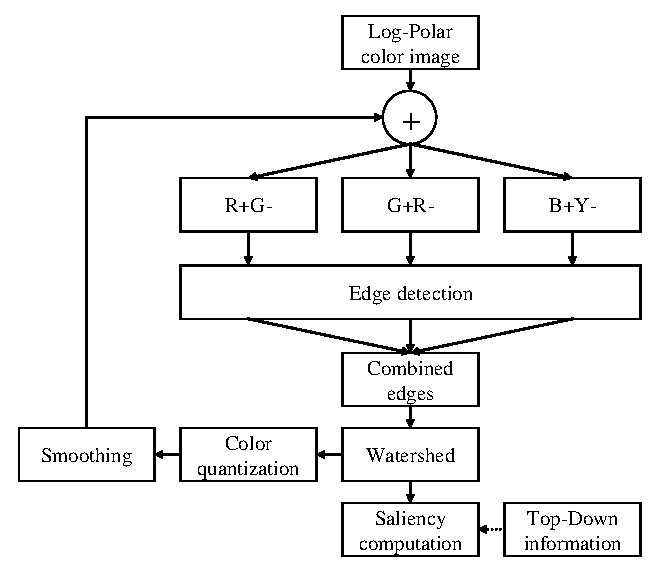
\includegraphics[width=0.6\linewidth]{./figs/attention/schema}
    \caption{Block diagram of the model. The input image is first separated in
     the three color opponency maps, then edges are extracted. A watershed transform
     creates the proto-objects on which the saliency is calculated,
     taking into account top-down biases.}
     \label{fig:model_diagram}
  \end{center}
\end{figure}

\subsection{Log-polar images}
The input is a sequence of color log-polar images \cite{SandiniT80,SandiniQSM00}.
The use of log-polar images comes from the
observation that the distribution of the cones, \ie the
photoreceptors of the retina involved in diurnal vision,
is not uniform. Cones have a higher density
in the central region called fovea (approximately $2^\circ$ of
the visual field), while they are sparser in the
periphery.
This distribution influences the
scanpaths during a visual search task \cite{WolfeG96} and so it has to
be taken into account to better model overt visual
attention. The log-polar mapping are in fact a model of the topological
transformation of the primate visual pathways from the
cartesian image coming from the retina to the visual cortex, taking also into
consideration the space-variant resolution of the retinal images.
This transformation that can be well
described as a logarithmic-polar (log-polar) mapping \cite{SandiniT80}.
Figure \ref{fig:logpolar_ex} shows an example Cartesian image and its
log-polar counterpart.

The main advantage of log-polar sensors is related to the small
number of pixels and the comparatively large field of view.
In fact the lower resolution of the periphery reduces the
images' size and thus reduces the computational load of the
visual processing, while the high resolution center can be
used for standard visual algorithms.

%From the mathematical point of view the log-polar
%mapping can be expressed as a transformation between
%the polar plane $(\rho,\theta)$ (retinal plane) and the log-polar
%plane $(\eta,\xi)$ (cortical plane) as follows \cite{SandiniT80}:
%\begin{equation}
%\left\{ 
%\begin{array}{l}
%	\eta=q\cdot\theta\\
%	\xi=log_a \frac{\rho}{\rho_0}
%\end{array}
%\label{eq:lp1}
%\right.
%\end{equation}
%\noindent where $\rho_0$ is the radius of the innermost circle, $1/q$ is the
%minimum angular resolution of the log-polar layout
%and $(\rho,\theta)$ are the polar co-ordinates.
%These are related
%to the conventional Cartesian reference system by:
%\begin{equation}
%\left\{ 
%\begin{array}{l}
%	x=\rho\cdot cos \theta\\
%	x=\rho\cdot sin \theta
%\end{array}
%\right.
%\label{eq:lp2}
%\end{equation}

\begin{figure}[]
	\begin{center}
		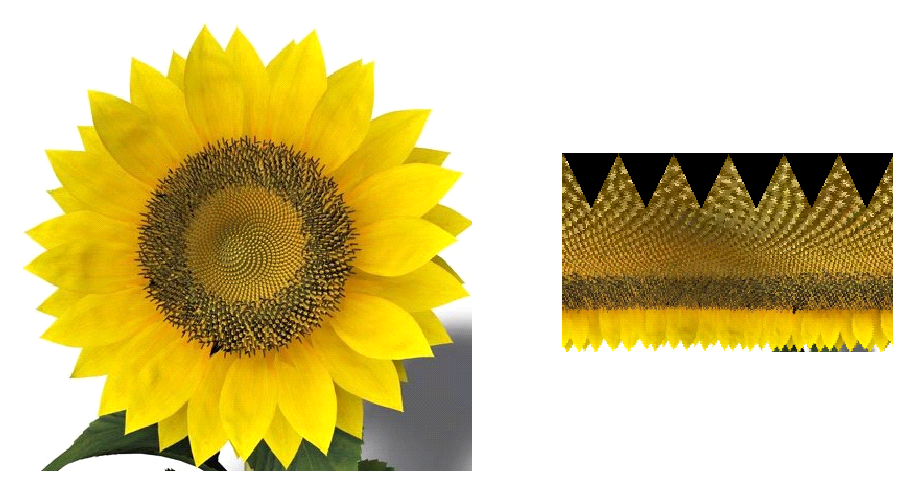
\includegraphics[width=0.8\linewidth]{./figs/attention/logpolarmapping2}
    \caption{Log-polar transform of an image.
    It is worth noting that the flower's petals, that have a polar structure,
    are mapped vertically in the log-polar image. Circles, on the other
    hand, are mapped horizontally. Furthermore, the stamens that lie in the
    center of the image of the flower, occupy about half of the
    corresponding log-polar image.}
  	\label{fig:logpolar_ex}
	\end{center}
\end{figure}

\subsection{Feature extraction}
As a first step the input image at time $t$ is averaged
with the output of a color quantization procedure (see
later) applied to the image at time $t-1$. This is to reduce
the effect of the input noise. The red, green, blue
channels of each image are then separated, and the
yellow channel is constructed as the arithmetic mean
of the red and green channels. Successively these four
channels are combined to generate three color
opponent channels, similar to those of the retina. Each
channel, normally indicated as $R^+G^-$, $G^+R^-$, $B^+ Y^-$,
has a center-surround receptive field (RF) with
spectrally opponent color responses. That is, for
example, a red input in the center of a particular RF
increases the response of the channel $R^+G^-$ , while a
green one in the surrounding will decrease its
response. The spatial response profile of the two sub-regions
of the RF, `center' and `surround', is expressed by a Gaussian,
hence resulting in a Difference-of-Gaussians (DoG).
A response is computed as there was a RF centered on
each pixel of the input image, thus generating an
output image of the same size of the input. This
operation, considering for example the $R^+G^-$ channel
is expressed by:
\begin{equation}
	R^+G^-(x,y)=\alpha \cdot R * g_c - \beta \cdot G * g_s
	\label{eq:dog}
\end{equation}
The two Gaussian functions, $g_c$ and $g_s$, are not
balanced: the ratio $\beta / \alpha$ is chosen equal to $1.5$,
consistent with the study of Smirnakis \etal \cite{SmirnakisBWBM97}. The
unbalanced ratio preserves the achromatic information:
that is, the response of the channels to a uniform gray
area is not zero. Hence the model does not need to
process achromatic information explicitly since it is
implicitly encoded, similarly to what happens in the
human retina's P-cells \cite{Billock95}. The ratio $\sigma_s / \sigma_c$, the
standard deviation of the two Gaussian functions, is
chosen equal to 3. To be noted that by filtering a log-polar
image with a standard space-invariant filter leads
to a space-variant filtered image of the original
cartesian image \cite{MallotSG90}.
Edges are then extracted on the three channels
separately using a generalization of the Sobel filter due
to \cite{LiYYY03}, obtaining $E_{RG}(x,y)$, $E_{GR}(x,y)$ and $E_{BY}(x,y)$. A
single edge map is generated combining the tree
outputs with a point-wise $\max(\cdot)$ operator:
\begin{equation}
	E(x,y)=\max\left\{\left|E_{RG}(x,y)\right|,\left|E_{GR}(x,y)\right|,\left|E_{BY}(x,y)\right|\right\}
	\label{eq:edge_map}
\end{equation}
%The log-polar transform has the side effect of
%sharpening the edges near the fovea due to the
%magnification factor of the mapping; this is
%compensated multiplying each pixel by a factor which
%is exponential on the eccentricity.

\subsection{Proto-objects}
\label{sec:att_protoobj}
It has been speculated, that synchronizations of visual
cortical neurons might serve as the carrier for the
observed perceptual grouping phenomenon \cite{EckhornBJBKMR88,GrayKES89}.
The differences in the phase of oscillation among
spatially neighboring cells are believed to contribute to
the segmentation of different objects in the scene.
We have used a watershed transform (rainfalling
variant) \cite{Smet00} on the edge map to simulate the result of
this synchronization phenomenon and to generate the
proto-objects.
The intuitive idea underlying the watershed transform comes from
geography: a topographic relief is flooded by water,
watershed are the divide lines of the domains of
attraction of rain falling over the region. In our view
the watershed transform simulates the parallel spread
of the activation on the image, until this procedure fills
all the spaces between edges. Differently from other
similar methods the edges themselves will never be
tagged as blobs and the method does not require
complex membership functions either. Moreover the
result does not depend on the order in which the points
are examined like in standard region growing \cite{WanH03}. As
a result, the image is segmented into blobs with either
uniform or uniform gradient of color. Hence from the choice
of the feature maps comes our definition of proto-objects
as closed areas of uniform color of the image.
A color quantized image is formed averaging the color inside
each blob. The result is blurred with a
Gaussian filter and stored: this will be used to perform
a time-smoothing by simple averaging with the frame
at time $t+1$ to reduce the effect of noise and increase
the temporal stability of the blobs. After an initial
startup time of about five frames, the number of blobs
and their shape stabilize. If any motion is detected in
the image then the smoothing procedure is halted and the
bottom-up saliency map becomes the motion image.

A feature or a stimulus
catches the attention if it differs from its
immediate surrounding. To replicate this phenomenon in the system
we compute a measure of bottom-up salience as the Euclidean distance in the
color opponent space between each blob and its
surrounding. However the size of the spot or focus of attention
should not be constant: it should change depending on the size of the
objects in the scene. To account for this fact the greater
part of the visual attention models in literature uses a
multi-scale approach filtering with some type of `blob'
detector (typically a DoG filter) at
various scales \cite{IttiK01}. We reasoned that this approach
lacks continuity in the choice of the size of the focus of
attention (see for example Figure \ref{fig:multiscale}).
We propose instead to dynamically vary the
region of interest depending on the size of the blobs.
That is the salience of each blob is calculated in
relation to a neighborhood proportional to its size. In
our implementation we consider a rectangular region 3
times the size of the bounding box of the blob as
surrounding region, centered on each blob. The choice
of a rectangular window is not incidental: filters
over rectangular regions can be
computed efficiently by employing the integral image
as in \cite{ViolaJ04}.

The bottom-up saliency is thus computed as:
\begin{eqnarray}
	S_{bottom-up}=\sqrt{\Delta RG^2 + \Delta GR^2+ \Delta BY^2} \\
	\Delta RG={\langle R^+G^- \rangle}_{blob} - {\langle R^+G^- \rangle}_{surround} \\
	\Delta GR={\langle G^+R^- \rangle}_{blob} - {\langle G^+R^- \rangle}_{surround} \\
	\Delta BY={\langle B^+Y^- \rangle}_{blob} - {\langle B^+Y^- \rangle}_{surround}
	\label{eq:s_bu}
\end{eqnarray}
\noindent where $\langle \rangle$ indicates the average of the image values
over a certain area (indicated in the subscripts).
The top-down influence on attention is, at the
moment, calculated in relation to the task of visually
searching for a given object. In this situation a model of
the object to search in the scene is given and this information is used to bias the saliency
computation procedure. In practice, the top-down
saliency map, $S_{top-down}$, is computed as the Euclidean distance in
the color opponent space, between each blob's average
color and the average color of the target, with a formula
similar to (\ref{eq:s_bu}).
%\begin{eqnarray}
%	S_{top-down}=\sqrt{\Delta RG^2 + \Delta GR^2+ \Delta BY^2} \\
%	\Delta RG={\langle R^+G^- \rangle}_{blob} - {\langle R^+G^- \rangle}_{object} \\
%	\Delta GR={\langle G^+R^- \rangle}_{blob} - {\langle G^+R^- \rangle}_{object} \\
%	\Delta BY={\langle B^+Y^- \rangle}_{blob} - {\langle B^+Y^- \rangle}_{object}
%	\label{eq:s_td}
%\end{eqnarray}
%\noindent with a notation similar to the one above.
Blobs that are too small or too big in relation to the
size of the images are discarded from the
computation of salience with two thresholds. The blob in
the center of the image (currently fixated) is also ignored
because it cannot be the target of the next fixation.
The total salience is simply calculated as the linear
combination of the top-down and bottom-up
contributions:
\begin{equation}
	S=k_{td} \cdot S_{top-down}+k_{bu} \cdot S_{bottom-up}
	\label{eq:s_tot}
\end{equation}
The center of mass of the most salient blob is selected for the next
saccade.

%An example of the intermediate and final
%maps of bottom-up salience is shown in Figure \ref{fig:maps_ex}.
%All the computations are done on log-polar images, but
%input and output images are shown remapped to
%cartesian for clarity.

\begin{figure}[]
  \begin{center}
    \begin{tabular}{cc}
       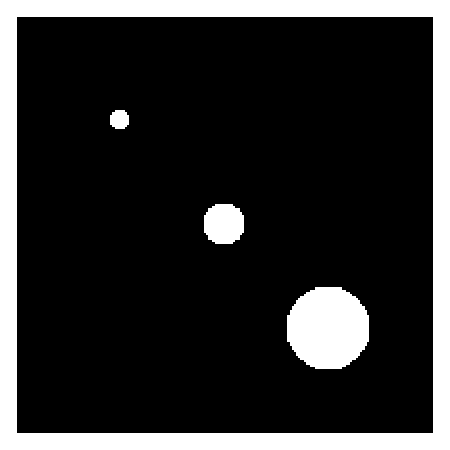
\includegraphics[width=0.37\textwidth]{figs/attention/dog1} &
       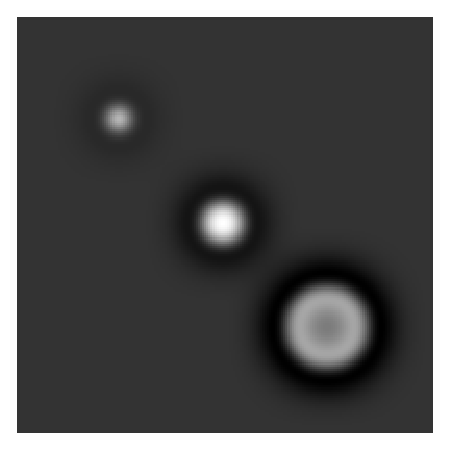
\includegraphics[width=0.37\textwidth]{figs/attention/dog2}
    \end{tabular}
    \caption{\label{fig:multiscale}Filtering the image on the left
     with a Difference-of-Gaussians, with the size of positive lobe
     equal to the circle in the middle, we obtain the
     image on the right. Smaller blobs will be depressed while larger
     ones will be depressed in their centers.}
  \end{center}
\end{figure}

%\begin{figure}[t]
%\begin{center}
%	\includegraphics[width=0.8\linewidth]{./figs/attention/schema_imm4}
%\end{center}
%  \caption{Example of model maps.}
%\label{fig:maps_ex}
%\end{figure}

\subsection{Inhibition of return}
In order to avoid being redirected immediately to a
previously attended location, a local inhibition is
transiently activated in the saliency map. This is called
`inhibition of return' (IOR) and it has been
demonstrated in human visual psychophysics.
%Posner and Cohen \cite{PosnerC84}, for example,
%demonstrated that the IOR does not seem to work
%in retinal coordinates but it is instead represented
%in an allocentric reference frame. Together with Klein
%\cite{Klein88}, they proposed that the IOR is required
%to allow an efficient visual search by discouraging
%shifting the attention toward locations that have
%already been inspected. Static scenes, however, are
%seldom encountered in real life: objects move and a
%``tagging system'' that merely inhibited environmental
%locations would be almost useless in any real situation.
In particular Tipper \cite{Tipper91} was among the firsts to
demonstrate that the IOR could be attached to moving objects.
%and this finding has been replicated and extended ever
%since \cite{AbramsD94,GibsonE94,Tipper94}.
Hence the IOR works by anchoring tags to
objects as they move; in other words this process seems
to be coded in an object-based reference frame.

Our system implements a simple object-based IOR.
A list of the last five positions visited is
maintained in a head-centered coordinate system and
updated with a FIFO (First In First Out) policy. The
position of the tagged blob is stored together with the
information about its color. When the robot gaze
moves --- for example by moving the eyes and/or the
head --- the system keeps track of the blobs it has
visited. These locations are inhibited only if they show
the same color seen earlier: so in case an inhibited
object moves or its color changes, the location
becomes available for fixation again.

%\begin{figure}[]
%  \begin{center}
%    \includegraphics[width=0.8\linewidth]{./figs/attention/schema_fasi}
%  \end{center}
%  \caption{The flow chart of the visual search of an object
%   (the toy airplane). The saliency
%   map is generated using the information about the color blue of
%   the toy.}
%  \label{fig:flow_chart}
%\end{figure}

\section{Results on sample images}
\label{sec:att_results}
The experiments reported here were carried out
on a robotic platform called Babybot. This is a
humanoid upper torso which consists of a head, an arm
and a hand. 
From the point of view of the sensors, the head is
equipped with two space-variant cameras \cite{SandiniQSM00}
and two microphones for visual and auditory feedback.
More details about the Babybot can be found in \cite{Natale04}.

Two examples of the saliency map are shown in
Figure \ref{fig:out_ex}: in \ref{fig:out_ex}.4 there is a purely bottom-up ($k_{td}=0$,
$k_{bu}=1$ in Equation (7)) map which is the result of the
processing of the scene in \ref{fig:out_ex}.1; in \ref{fig:out_ex}.5 there is a purely
top-down ($k_{td}=1$, $k_{bu}=0$) map output after the
processing of \ref{fig:out_ex}.2. In the latter the robot was instructed
to search for the toy airplane.
%After a saccade on the
%object and a successfully recognition the figure-ground
%segmentation is shown in Figure \ref{fig:out_ex}.6.

%We have tested the attention system while guiding
%the recognition and grasping of objects in the Babybot.
%In table \ref{table:att_ris}, results are shown when using a toy car and
%a toy airplane as target objects; 50 training/visual search sessions
%were performed for each object. The first column shows
%the recognition rate, the second the average number
%of saccades (mean $\pm$ standard deviation) it takes the
%robot to locate the target in case of successful recognition.

%\begin{table*}
%\caption{Performance of the recognition system measured from a set of 50 trials.}
%\begin{center}
%\begin{tabular}[!h]{|l|c|c|}
%\hline
%  Object      & Recognition & Number of saccades \\
%              & rate        & when recognized    \\ \hline
%  Toy car     & $94\%$      & $3.19\pm2.17$      \\
%  Toy airplane & $88\%$      & $3.02\pm2.84$      \\ \hline
%\end{tabular}
%\end{center}
%\label{table:att_ris}
%\end{table*}

In order to compare the performance of the system
with the state of the art model of Itti, we
have done a comparison test of the bottom-up attention
using the database of images by Itti and Koch \cite{IttiK01b} (color
images with an emergency triangle and relative binary
segmentation masks of the triangle), which is freely
available on the Internet\footnote{\url{http://ilab.usc.edu/imgdbs/}, last access 30/05/2007.}.
First, the original images and segmentation masks are
cropped to a square and transformed to the log-polar
format (see Figure \ref{fig:itti_ex}.1 and Figure \ref{fig:itti_ex}.2
for the cartesian remapped images). To simulate the
presence of a static camera, the images are presented to
the system continuously and, after five `virtual'
frames, the bottom-up saliency map is confronted with
the mask. In $49\%$ of the images a point inside the
emergency triangle is selected as the most salient
(see an example in Figure \ref{fig:itti_ex}.3). It is worth noting that a
direct comparison with the results of Itti and Koch in \cite{IttiK01b}, by
counting the number of false detection before the
target object is found, is not possible since after each
saccade the log-polar image changes a lot.

Often models of visual attention are usually used as
sort of filters for object recognition systems, as in, \eg, \cite{WaltherK06}.
In such systems the attention model and the object recognition one
live in two different `worlds': they work on two
different representations of the input images and few or none
of the computation done by the first stage is used by the
second one. A proof of concept on how to build an object
recognition system on the same basis of the visual attention,
that is on the concept of proto-objects was presented in
\cite{Orabona07}. The visual attention system and the object recognition
system were also used to guide the grasping action of the robot.


\begin{figure}[!h]
  \begin{center}
    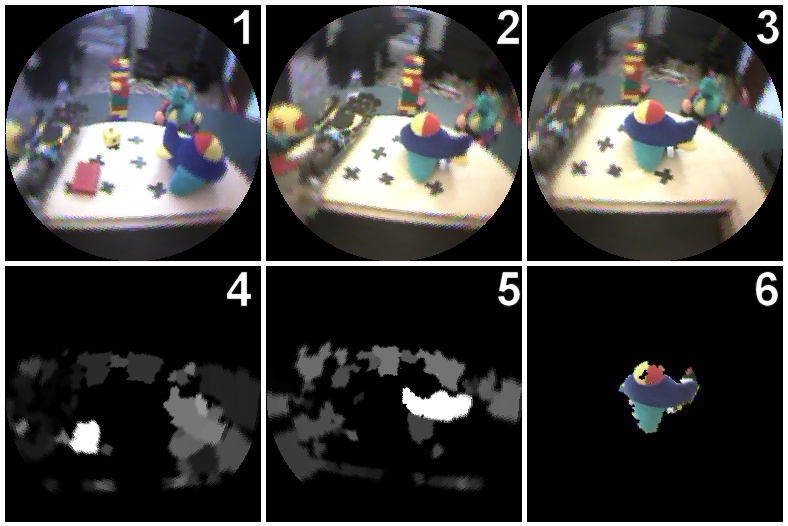
\includegraphics[width=0.9\linewidth]{./figs/attention/a3}
    \caption{Example saliency maps. $(c)$ is the 
     bottom-up saliency map of the image $(a)$. $(d)$ is the top-down
	   saliency map of $(b)$, while searching for the blue
	   toy airplane.}
    \label{fig:out_ex}
  \end{center}
\end{figure}

\begin{figure}[!h]
  \begin{center}
    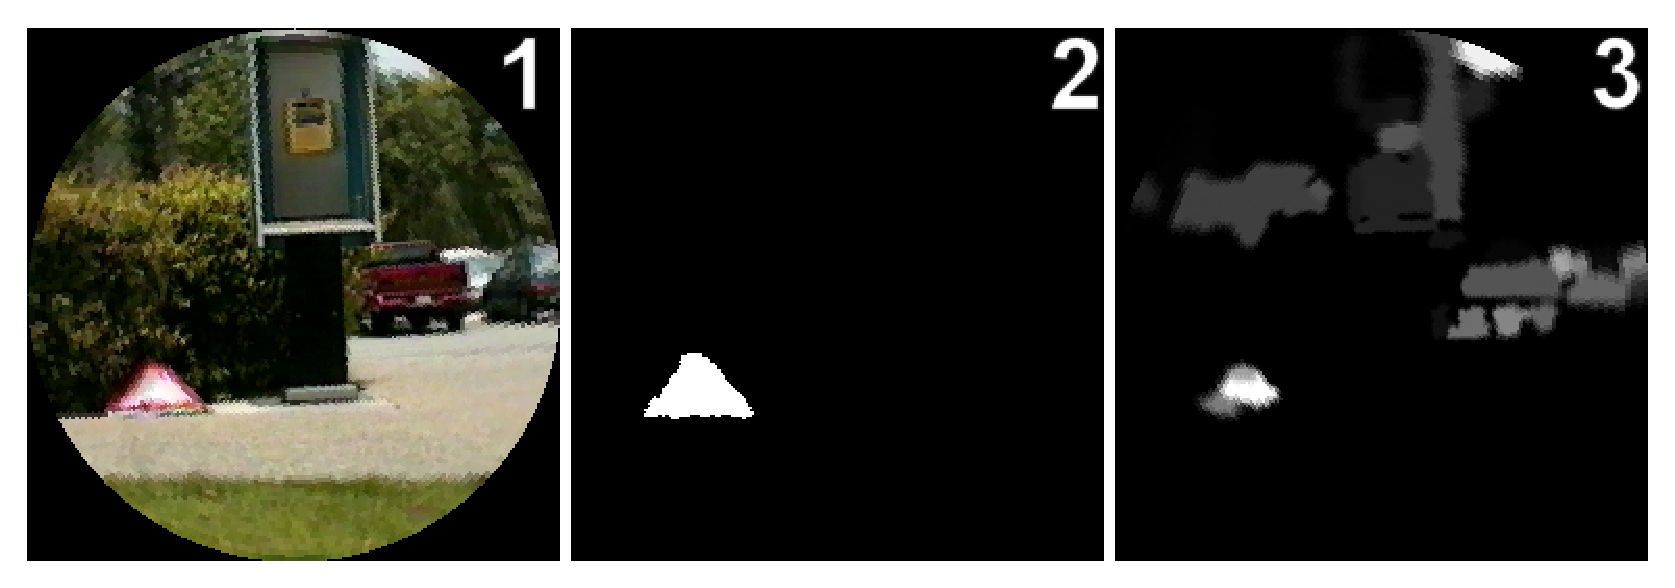
\includegraphics[width=0.9\linewidth]{./figs/attention/itti}
    \caption{Result on a sample image taken from \cite{IttiK01b}.
     (1) is the log-polar input image and (2) the corresponding taget binary mask.
     (3) is the bottom-up saliency map.}
    \label{fig:itti_ex}
  \end{center}
\end{figure}


\section{A better definition of proto-objects}
\label{sec:ass_fields}

%As said in the introduction, it is important to stress the fact
%that visual attention is not just a stand-alone module existing
%in our brains, but a part of a complex interconnected system
%that allows us complex action in our environment.

As said above, object-based theories of attention stress the importance
of a sort of segmentation of the visual input in coherent regions.
On the other hand the term `grouping' (or `segmentation')
is a common concept in the long research history of perceptual grouping
by the Gestalt psychologists.
Back at the beginning of the last century they
described, among other things, the ability of the human
visual system to organize parts of the retinal stimulus
into `Gestalten', that is, into organized structures.
A number of so-called Gestalt laws 
(proximity, common fate, good continuation, closure, \etc) were
formulated that are believed to govern our perception.

Nowadays the more typical view of such grouping
demonstrations would be that they reflect non-arbitrary properties within the stimuli
(similarity, common motion, \etc), which the visual system
exploits heuristically because these properties
are likely to reflect divisions into distinct objects in the real world.
In particular these properties work because they reflect characteristics of
the real world. 
In this sense it should be possible to learn these heuristic
properties and hence to learn from the images better rules
to build the proto-objects.


\subsection{Learning the association fields}
%Previous studies have shown that it is possible to learn
%certain properties of the responses of the neurons of the
%visual cortex, as for example the receptive fields of
%complex and simple cells, through the analysis of the
%statistics of natural images and by employing principles
%of efficient signal encoding from information theory, \eg \cite{Bell97}.
%Here we want to go further and consider how the output
%signals of `complex cells' are correlated and which
%information is likely to be grouped together.
%We want to learn `association fields', which are a
%mechanism to integrate the output of filters with
%different preferred orientation, in particular to
%link together and enhance contours, and in the end to create our
%perception of proto-objects.

% We used static
%natural images as training set and the tensor notation
%to express the learned fields. Finally we tested these
%association fields in a computer model to measure their
%performance.

%This chapter is organized as follows: section \ref{sec:ass_gestalt}
%introduces the idea of the link between the Gestalt laws and the
%statistics of the world. Section \ref{sec:ass_learning}
%contains a description of the method, and section \ref{sec:ass_pre_res}
%describes a first set of experimental results and a method to
%overcome problems due to the non-uniform distribution of the
%image statistics. In section \ref{sec:ass_res} we show the fields
%computed with this last modification and finally in sections
%\ref{sec:ass_using} and \ref{sec:ass_disc} we show the performance
%of the fields in edge detection on a database of natural images and
%we draw some conclusions.


%\section{Gestalt laws, statistics and neurons}
%\label{sec:ass_gestalt}
%The goal of perceptual grouping in computer vision is
%to organize visual primitives into higher-level primitives
%thus explicitly representing the structure contained in
%the data.
%The idea of perceptual grouping for computer
%vision has its roots in the well-known work of the Gestalt
%psychologists back at the beginning of the last century
%who described, among other things, the ability of the human
%visual system to organize parts of the retinal stimulus
%into ``Gestalten'', that is, into organized structures.
%They formulated a number of so-called Gestalt laws
%(proximity, common fate, good continuation, closure, \etc)
%that are believed to govern our perception. It is logical
%to ask if these laws are present in the statistics of the world.

%On the other hand it has been long hypothesized that the early visual system is adapted to the input statistics \cite{Barlow61}. Such an adaptation is thought to be the result of the joint work of evolution and learning during development. Neurons, acting as coincidence detectors, can discover and use regularities in the incoming flow of sensory information, which eventually represent the Gestalt laws. It has been proposed that, for example, the mechanism that link together the elements of a contour is rooted in our biology, with neurons with lateral and feedback connections implementing these laws.

There is a large body of literature about computational modeling
of various parts of the visual cortex, starting from the assumption that
certain principles guide the neural code (\cite{SimoncelliO01} for a review).
In spite of this, there is very little literature on learning an entire
hierarchy of features, that is not only the first layer, and possibly
starting from these initial receptive fields.

A first step in the implementation of these laws are the `association fields'
\cite{FieldHH93}. These fields are supposed to resemble the pattern of
excitatory and inhibitory lateral connection between different orientation
detector neurons as found, for instance, by Schmidt \etal \cite{SchmidtGLS97}.
In fact, Schmidt has shown that cells with an orientation preference in area
17 of the cat are preferentially linked to iso-oriented cells. Furthermore,
the coupling strength decrease with the difference in the preferred
orientation of pre- and post-synaptic cell.

In the literature, association fields are often hand-coded and employed in
many different models with the aim to reproduce the human performance in
contour integration. Models typically consider variations of the co-circular
approach \cite{Grossberg85,Guy96,Li98}, which states that two oriented elements are
very likely part of the same curve if they are tangent to the same circle.
Our approach is instead to try to to learn these
association fields directly from natural images, without any prior assumption.

%One of the first publication addressing second order relations
%of edge-like structures in images is from Kr{\"u}ger \cite{Kruger98}.
%Then different authors have used different approaches to try to ``learn'' this fields: using a database of tagged images \cite{ElderG02,Geisler01}, %using motion as an implicit tagger \cite{Prodohl01} or hypothesizing certain coding properties of the cortical layer \cite{Hoyer02}.

%Our approach is similar to to one of Sigman \etal \cite{Sigman01},
%which uses images as the sole input. Further, we aim to obtain
%precise association fields, useful to link contours in a computer model.

%\begin{figure}[]
%	\begin{center}
%		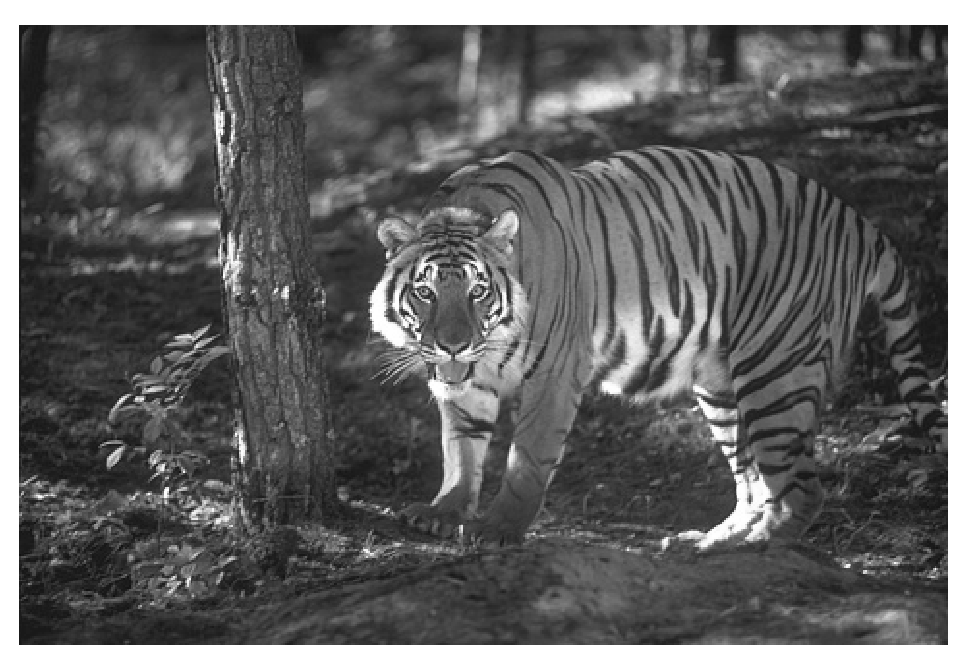
\includegraphics[width=0.8\linewidth]{./figs/af/esempio}
%	\end{center}
%  \caption{Sample input image from the Berkeley Segmentation Database.
%    All the images were converted to grayscale before using the proposed method.}
%	\label{fig:exampleimg}
%\end{figure}



%\section{Learning from natural images}
%\label{sec:ass_learning}

We assume the existence of a first layer that
simulates the behavior of the complex cells; in this
article we do not address the issue on how to learn
them since we are interested in the next level of the hierarchy.
Using the output of this layer we want to estimate the mean
activity around points with a given orientation.

To have a precise representation of the orientations and at the same time
something mathematically convenient, we have chosen to use the tensor notation.
Second order symmetric tensors can capture the information about the first
order differential geometry of an image. Each tensor describes both the
orientation of an edge and its confidence for each point. The tensor can be
visualized as an ellipse, whose major axis represents the estimated tangential
direction and the difference between the major and minor axis the confidence
of this estimate. Hence a point on a line will be associated with a thin
ellipse while a corner with a circle.
Consequently given the orientation of a reference pixel, we estimate the mean
tensors associated with the surrounding pixels. The use of the tensor notation
give us the possibility to exactly estimate the preferred orientation in each
point of the field and also to quantify its strength and confidence.

%We have chosen to learn a separate association field for each possible
%orientation.
%This is done for two main reasons:
%\begin{itemize}
%	\item It is possible to find differences between the association fields.
%	For example, it is possible to verify that the association field for the orientation of 0 degrees is
%	stronger than that of 45 degrees.
%	\item For applications of computer vision, considering the discrete nature of digital images,
%	it is better to separate the masks for each orientation, instead of combining the data in a single mask
%	that has to be rotated leading to sampling problems. The rotation can be done safely
%	only if there is a mathematical formula that represents the field, while on the other hand we are inferring the
%	field numerically.
%\end{itemize}

We have chosen to learn $8$ association fields, one for each discretized
orientation. The extension of the fields is chosen to be of $41$x$41$ pixels
taken around each point.
Even if we quantized the orientation of the (central)
reference pixel to classify the different fields, the information about the remaining
pixels in the neighbor were not quantized, differently other approaches, \ie \cite{Sigman01}.
There is neither a threshold nor a pre-specified number of bins for
discretization and thus we obtain a precise representation of the association fields.

Images used for the experiments were taken from the
publicly available database (Berkeley Segmentation
Database\footnote{\url{http://www.eecs.berkeley.edu/Research/Projects/CS/vision/grouping/segbench/}, last access 30/05/2007.}
\cite{MartinFTM01}) which consists of $300$
color images of $321$x$481$ and $481$x$321$ pixels;
$200$ of them were converted to black and white and used
to learn the fields; an
example image from the dataset is shown in Figure \ref{fig:exampleimg} $(a)$.


\begin{figure}[]
	\begin{center}
		\begin{tabular}{cc}
			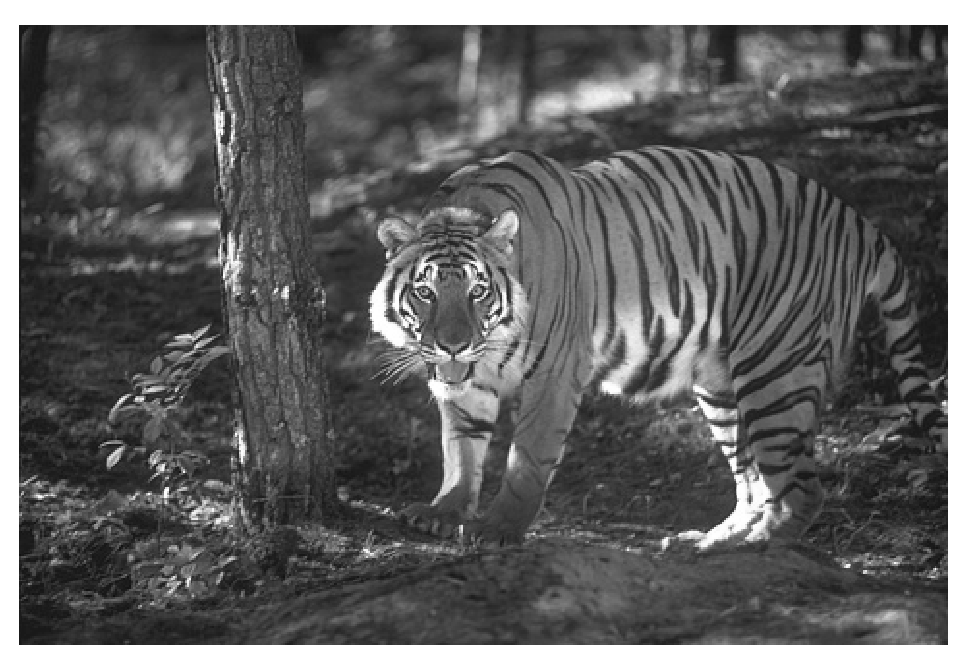
\includegraphics[width=0.4\linewidth]{./figs/af/esempio} &
			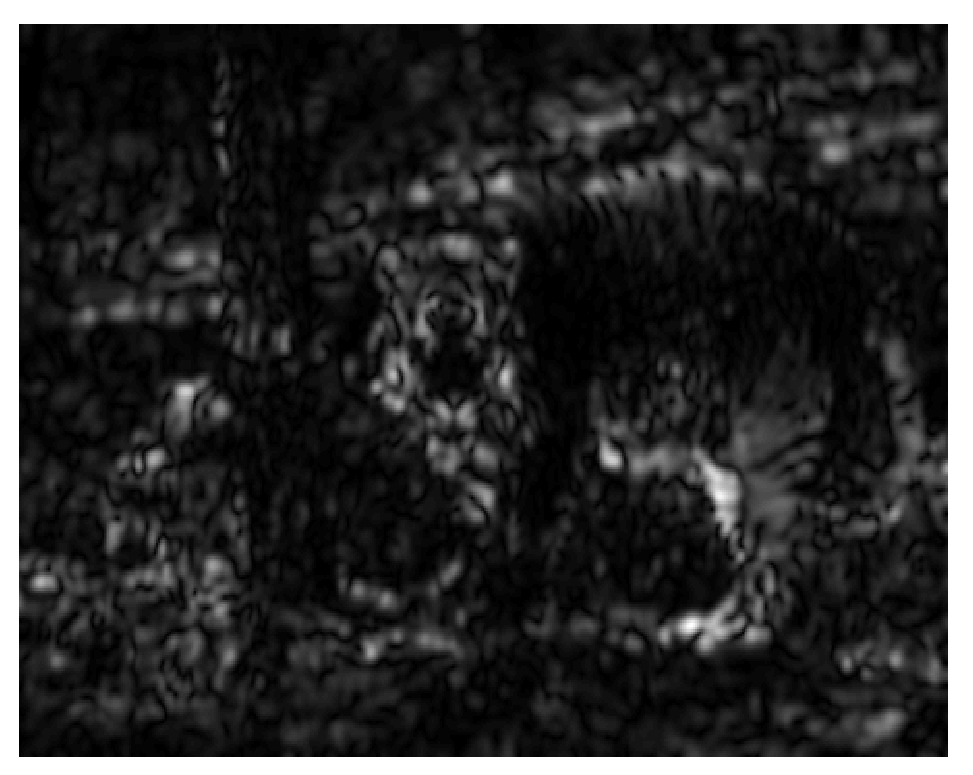
\includegraphics[width=0.4\linewidth]{./figs/af/esempio_fil} \\
			$(a)$ & $(b)$
		\end{tabular}
    \caption{$(a)$ Sample input image from the Berkeley Segmentation Database.
     All the images were converted to grayscale before using the proposed method.
     $(b)$ Complex cells output to the image in $(a)$ for $0^\circ$ filter of formula (\ref{eqn:nrgmod}).}
    \label{fig:exampleimg}
	\end{center}
\end{figure}


\subsection{Feature extraction stage}
\label{sec:ass_feature}
There are several models of the complex cells of V1, but we have chosen to
use the classic energy model \cite{Morrone88}.
The response is calculated as:
\begin{equation} \label{eqn:nrgmod}
E_\theta=\sqrt{\left(I*f^{e}_\theta \right)^2+\left(I*f^{o}_\theta \right)^2}
\end{equation}
where $f^{e}_\theta$ and $f^{o}_\theta$ are a quadrature pair of even- and
odd-symmetric filters at orientation $\theta$. Our even-symmetric filter is
a Gaussian second-derivative, and the corresponding odd-symmetric is its
Hilbert transform.
In Figure \ref{fig:exampleimg} $(b)$ there is an example of the output of the
complex cells model for the $0$ degrees orientation.

Then the edges are thinned using a standard non-maximum
suppression algorithm.
%This is equivalent to finding edges with a Laplacian
%of Gaussian and zero crossing.
The outputs of these filters are used to construct our local tensor
representation.



\subsection{Tensors}

%\begin{equation} \label{eqn:tensdef}
%{\mathcal T}=\left[
%\begin{array}{cc}
%a_{11} & a_{12} \\ a_{21} & a_{22}
%\end{array}
%\right]
%\end{equation}

In practice a second order tensor is denoted by a $2$x$2$ symmetric matrix.
It is constructed by direct summation of three quadrature filter pair output magnitudes as in \cite{Knutsson89}:
\begin{equation} \label{eqn:sumquad}
T=\sum^3_{k=1}E_{\theta_k}\left(\frac{4}{3}\hat{n}_k^T \hat{n}_k-\frac{1}{3}I\right)
\end{equation}
where $E_{\theta_k}$ is the filter output as calculated in (\ref{eqn:nrgmod}), $I$ is the 2x2 identity matrix and the filter directions $\hat{n}_k$ are:
\begin{equation} \label{eqn:fildir}
\begin{array}{lll}
\hat{n}_1=\left(1,0\right) \\
\hat{n}_2=\left(1/2,\sqrt{3}/2\right) \\
\hat{n}_3=\left(-1/2,\sqrt{3}/2\right)
%\hat{n}_2=\left(\frac{1}{2},\frac{\sqrt{3}}{2}\right) \\
%\hat{n}_3=\left(-\frac{1}{2},\frac{\sqrt{3}}{2}\right)
\end{array}
\end{equation}

The greatest eigenvalue $\lambda_1$ and its corresponding eigenvector $e_1$ of a tensor associated to a pixel represent respectively the strength and the direction of the main orientation. The second eigenvalue $\lambda_1$ and its eigenvector $e_1$ have the same meaning for the orthogonal orientation. The difference $\lambda_1-\lambda_2$ is proportional to the likelihood that a pixel contains a distinct orientation.

\subsection{The path across a pixel}
\label{sec:ass_pre_res}
We have run our test only for a single scale, choosing the $\sigma$ of the Gaussian filters
equal to $2$, since preliminary tests have shown that a similar version of the fields is obtained with other scales as well.
Two of the obtained fields are in Figure \ref{fig:field1}. It is clear that they are somewhat corrupted by the presence of horizontal and vertical orientations in any of the considered neighbors and by the fact that
in each image patch there are edges
that are not passing across the central pixel. On the other hand we want to learn association field for curves that do pass through the central pixel.

%Geisler \etal \cite{Geisler01} used a human labeled database
%of images to infer the likelihood of finding edges with a
%certain orientation relative to the reference point.
%On the other hand, Sigman \etal \cite{Sigman01} using only
%relative orientation and not absolute ones, could not have seen this problem.

%In our case
%we want to use unlabeled data to demonstrate that it is possible to
%learn from raw images and, as mentioned earlier, we do not want to
%consider only the relative orientations, but rather a different field for each
%orientation.

We believe that this is the same problem that Prod\"ohl \etal \cite{Prodohl01} experienced using static images: the learned fields supported collinearity in the horizontal and vertical orientations but hardly in the oblique ones. They solved this problem using motion to implicitly tag only the important edges inside each patch.

Once again the neural way to solve this problem can be the synchrony of the
firing between nearby neurons (see Section \ref{sec:att_protoobj})
Inspired by this we considered in each patch only pixels that belong to any
curve that goes through the central pixel. In this way the gathered data will
contain only information about curves connected to the central pixel.
Note that we select curves inside each patch, not inside the entire image.
The simple algorithm used to select the pixels in each patch is the following:
\begin{enumerate}
	\item put central pixel of the patch in a list;
	\item tag first pixel in the list and remove it from the list. Put surrounding pixels that are active (non-zero) in the list;
	\item if the list is empty quit otherwise go to $2$.
\end{enumerate}
With this procedure we remove the influence of horizontal and vertical edges that are more present in the images and
that are not removed by the process of averaging. On the other hand, we are losing some information, for example about parallel lines, that in any case should not be useful for the enhancement of contours.
Note that this method is completely parameter free; we are not selecting the curves following some specific criterion, instead we are just pruning the training set from some kind of noise.
It is important to note that this method will learn the bias present in natural images versus horizontal and vertical edges \cite{CoppolaPMP98}, but it will not be biased to learn \emph{only} these statistics, as in Prod\"ohl \etal \cite{Prodohl01} when using static images.
A similar approach has been used by \cite{Fitzpatrick03} to disambiguate the edges of a target object from the other of the environment, using self-caused motion.

\begin{figure}[h]
	\begin{center}
		\begin{tabular}{cc}
			\fbox{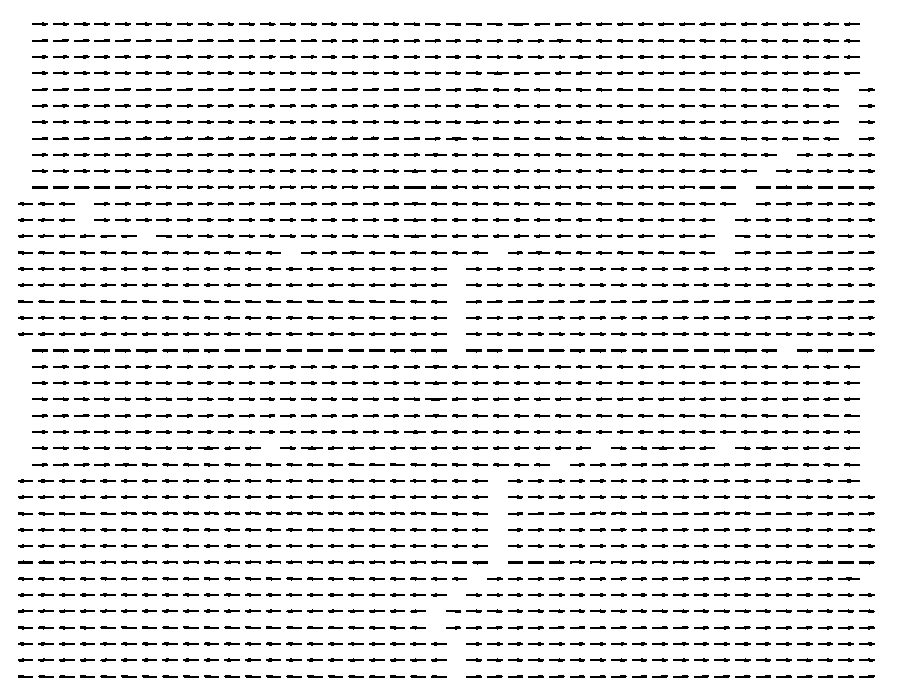
\includegraphics[width=0.4\linewidth]{./figs/af/or_ns_e1_1}} &
			\fbox{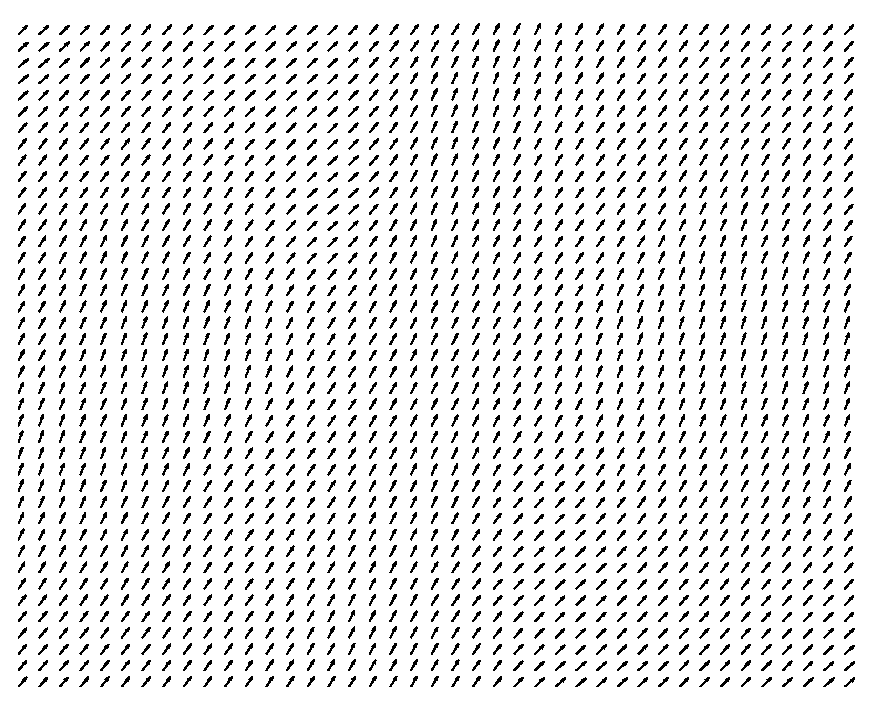
\includegraphics[width=0.4\linewidth]{./figs/af/or_ns_e1_4}} \\
			$(a)$ & $(b)$
		\end{tabular}
    \caption{Main directions for the association field for the orientation of 0 $(a)$ and 67.5 $(b)$ degrees in the central pixel.}
	  \label{fig:field1}
	\end{center}
\end{figure}

%\begin{figure}[]
%	\begin{center}
%		\fbox{
%			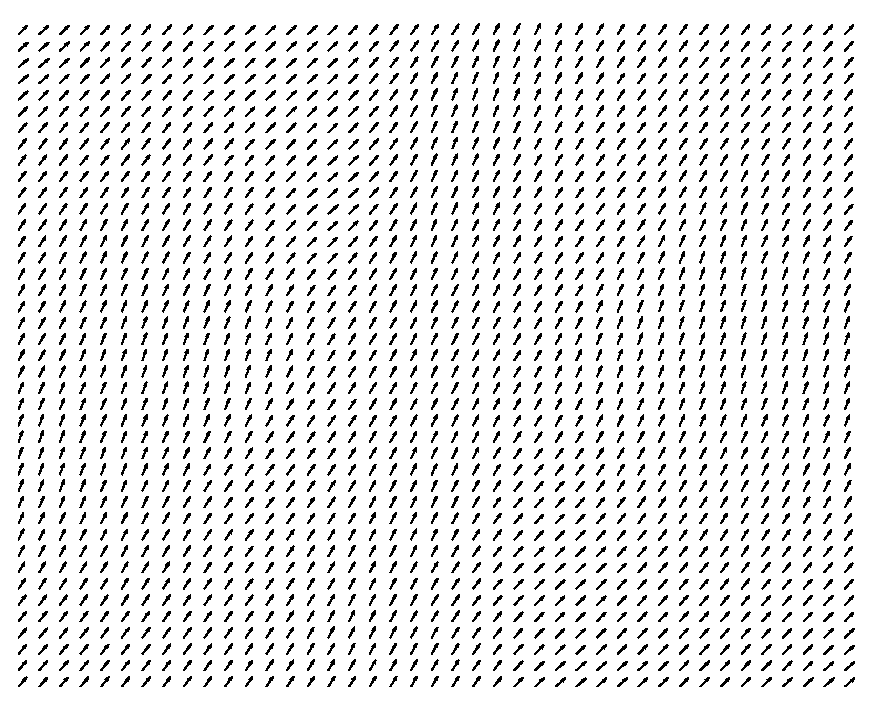
\includegraphics[width=0.8\linewidth]{./figs/af/or_ns_e1_4}
%		}
%	\end{center}
%  \caption{Main directions for the association field for the orientation of 67.5 degrees in the central pixel.}
%	\label{fig:field2}
%\end{figure}


\section{Validating the association fields}
\label{sec:ass_res}
%We tested the modified procedure on the database of natural images and also
%on random images (results not shown), to verify that the results were not an
%artifact due to the method.
In Figures \ref{fig:field1_e1_new} and \ref{fig:field1_l1l2_new} there are the
main orientations and their strengths (eigenvalues) of the mean estimated
tensors for the orientation of $0$ and $67.5$ degrees of the central pixel.
The structure of the obtained association field closely resembles the fields
proposed by others based on collinearity and co-circularity.
It is clear that the size of the long-range connection far exceeds the size of the
classical receptive field. Note that the noisier regions in the
orientation map corresponds to very small eigenvalues so they do not influence very
much the final result.

While all the fields have the same trend, there is a clear difference in the
decay of the strength of the fields. To see this we have considered only the
values along the direction of the orientation in the center, normalizing the
maximum values to one. Figure \ref{fig:conf} $(a)$ shows this decay.
It is clear that fields for horizontal and vertical edges have a wider support,
confirming the results of Sigman \etal \cite{Sigman01}.

The obtained fields can be used with any existing model of contour enhancement,
but to test them we have used the tensor voting scheme proposed by
Guy and Medioni \etal \cite{Guy96}. The choice is somewhat logical considering
to the fact that the obtained fields are already tensors. In the tensor voting
framework points communicate with each other in order to refine and derive the
most preferred orientation information.
%Differently to the original tensor
%voting algorithm we don't have to choose the right scale of the fields
%\cite{LeeM99} since it is implicitly in the learnt fields.
We compared the performances of the tensor voting algorithm using the learned
fields versus the simple output of the complex cell layer, using the Berkeley
Segmentation Database and the methodology proposed by Martin \etal
\cite{MartinFM04,MartinFTM01}. We can see the results in Figure
\ref{fig:conf} $(b)$: there is always an improvement using the tensor voting and
the learned association fields instead of just using the outputs of
the complex cells alone. An example of the results on the test image in
\ref{fig:exampleimg} $(a)$, after the non-maximum suppression procedure, are
shown in Figure \ref{fig:im_oe_pg}.

%\begin{figure}[]
%	\begin{center}
%		\fbox{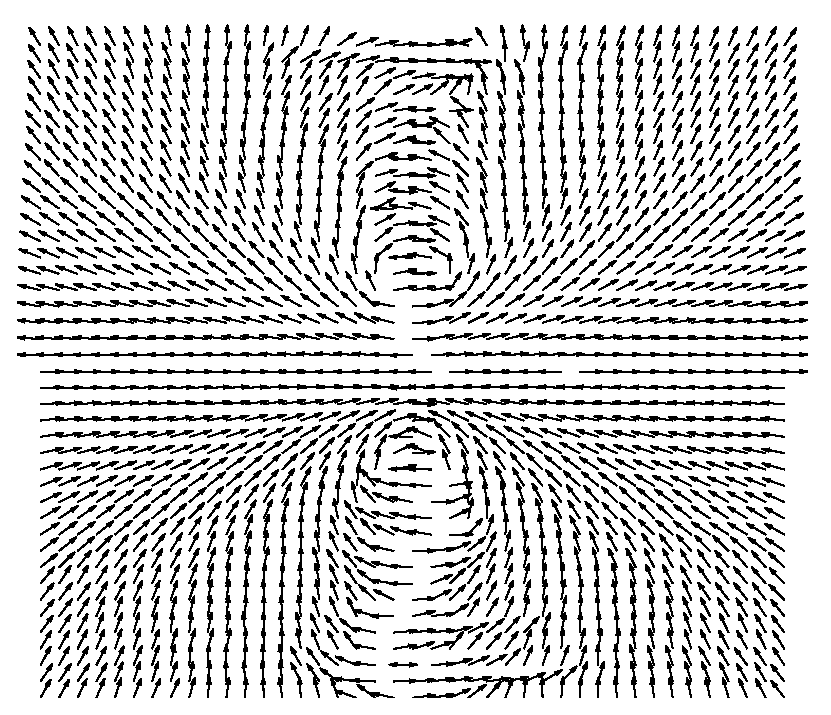
\includegraphics[width=0.8\linewidth]{./figs/af/or_e1_1}}
%	\end{center}
%  \caption{Main directions for the association field for the orientation of 0 degrees in the central pixel, with the modified approach.}
%	\label{fig:field1_e1_new}
%\end{figure}

\begin{figure}[h]
	\begin{center}
		\begin{tabular}{cc}
			\fbox{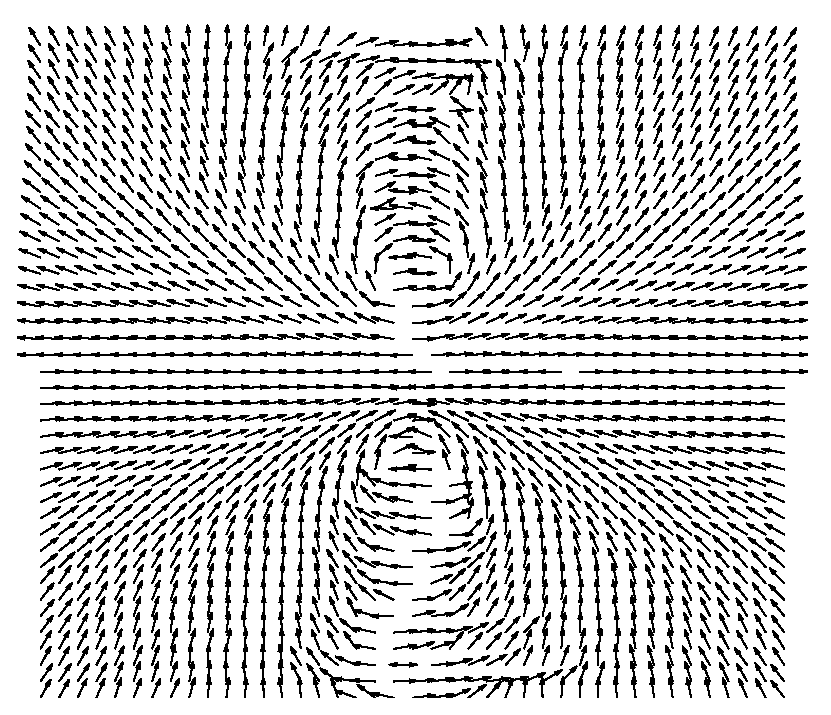
\includegraphics[width=0.4\linewidth]{./figs/af/or_e1_1}} &
			\fbox{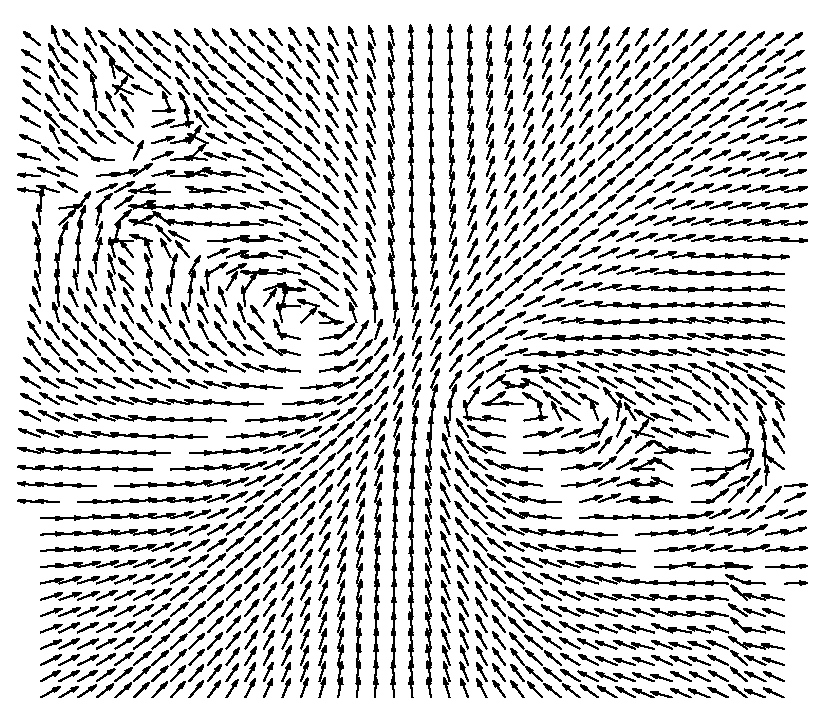
\includegraphics[width=0.4\linewidth]{./figs/af/or_e1_4}} \\
			$(a)$ & $(b)$
			%\fbox{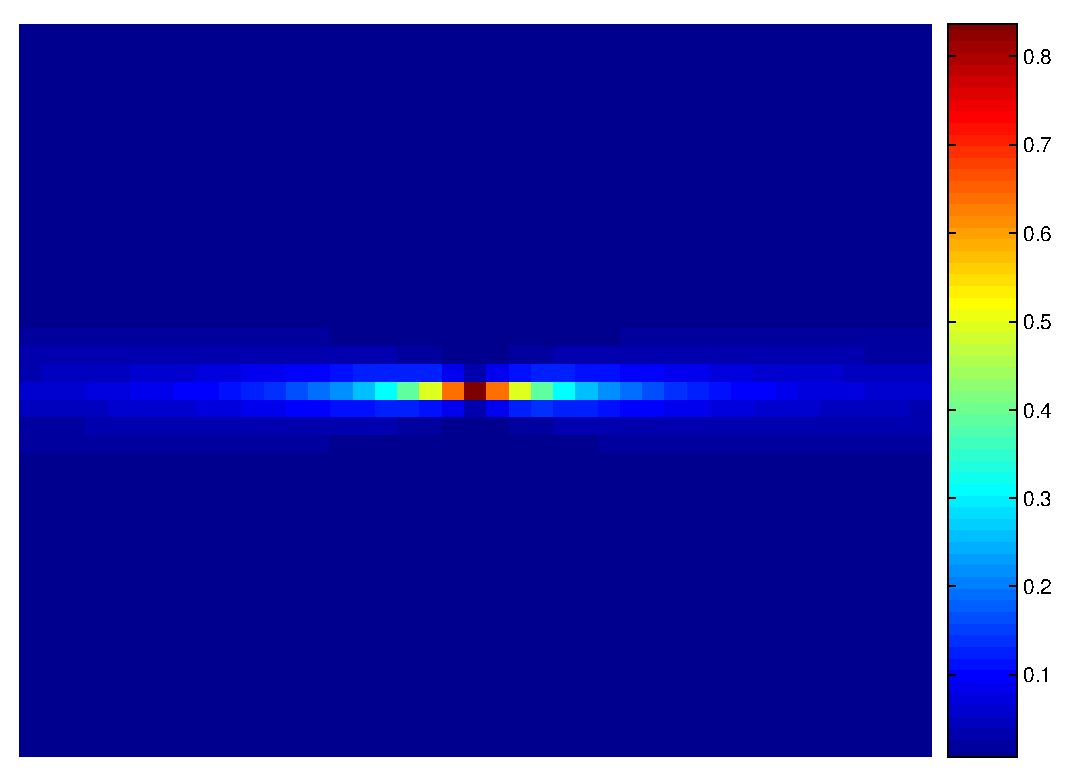
\includegraphics[width=0.45\linewidth]{./figs/af/or_l1l2_1}} &
			%\fbox{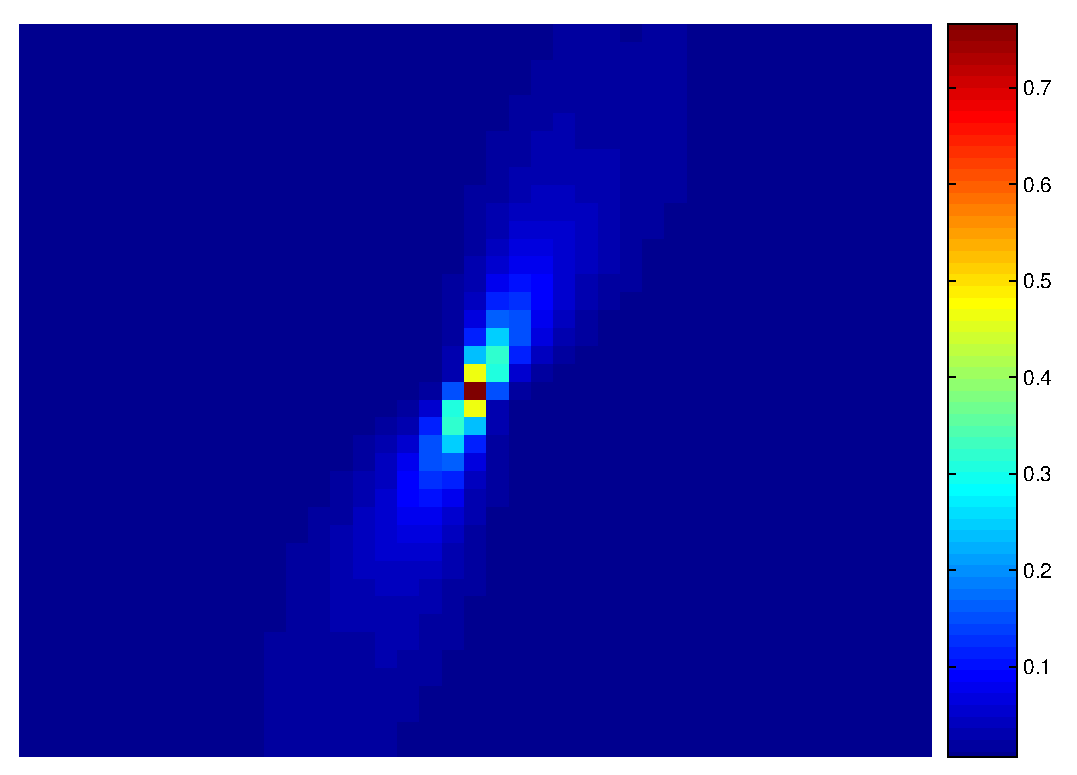
\includegraphics[width=0.45\linewidth]{./figs/af/or_l1l2_4}} \\
			%$(c)$ & $(d)$
		\end{tabular}	
    \caption{Main directions for the association field for orientation of $0^\circ$ $(a)$ and $67.5^\circ$ $(b)$, with the modified approach.}
	  \label{fig:field1_e1_new}
	\end{center}
\end{figure}

\begin{figure}[h]
	\begin{center}
		\begin{tabular}{cc}
			\fbox{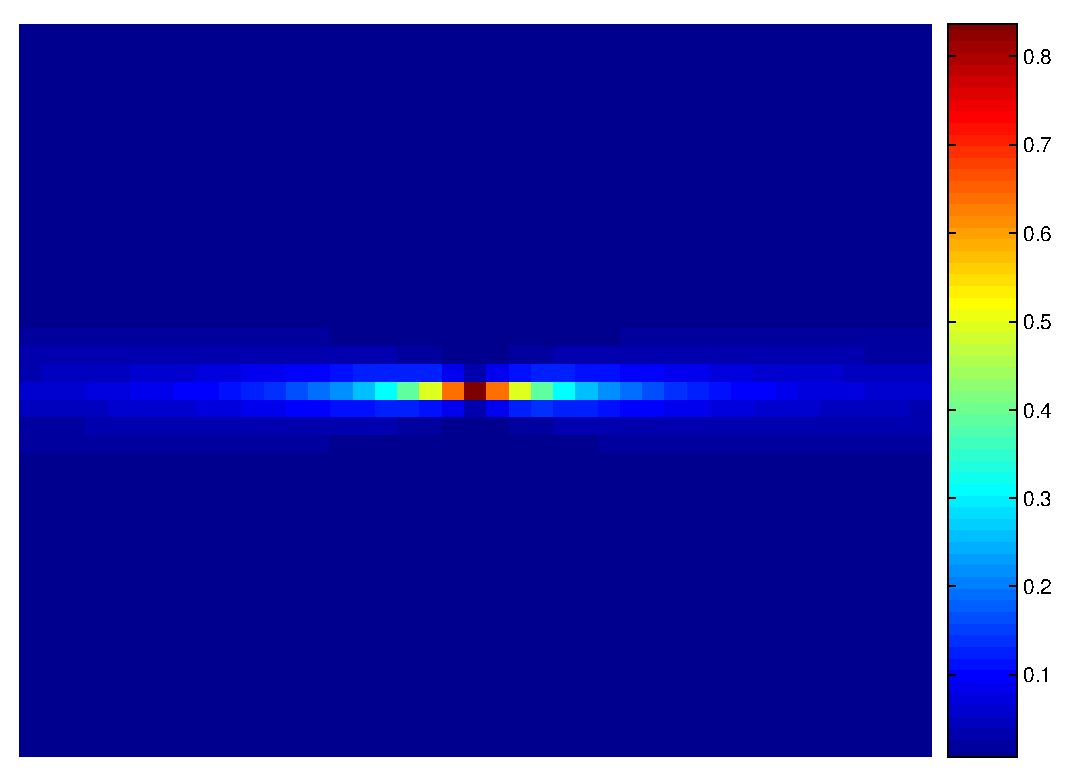
\includegraphics[width=0.4\linewidth]{./figs/af/or_l1l2_1}} &
			\fbox{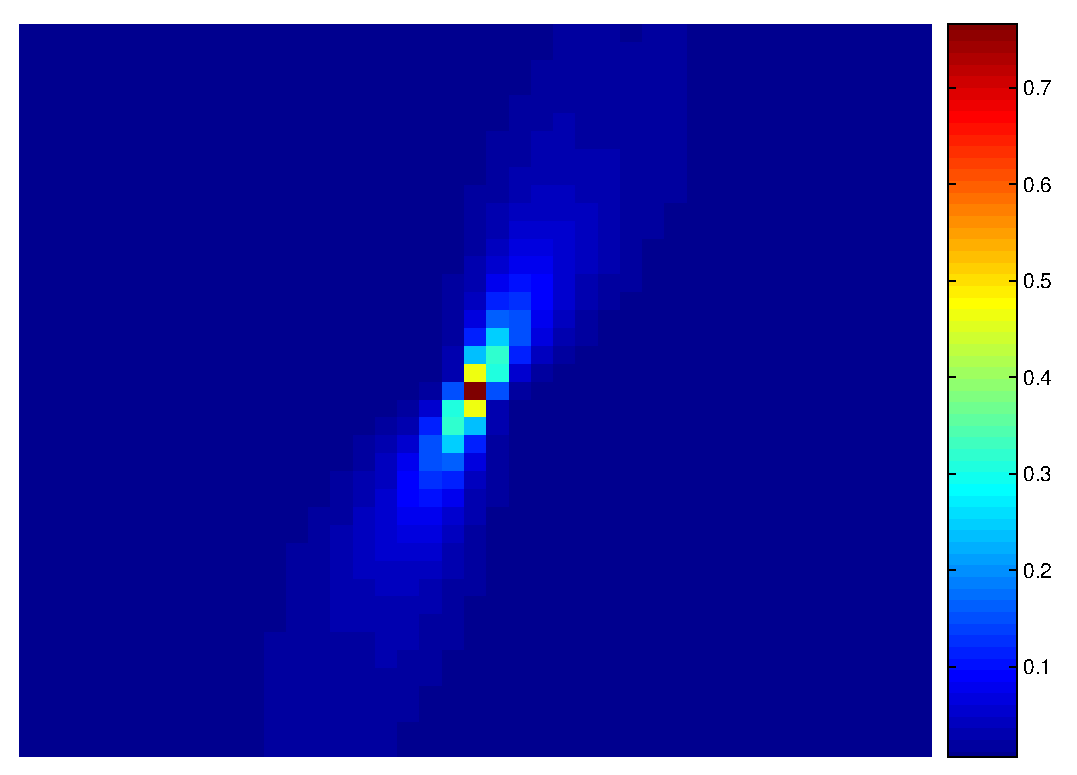
\includegraphics[width=0.4\linewidth]{./figs/af/or_l1l2_4}} \\
			$(a)$ & $(b)$
		\end{tabular}
	\end{center}
  \caption{Difference between the two eigenvalues of the association fields of Figure \ref{fig:field1_e1_new}.}
	\label{fig:field1_l1l2_new}
\end{figure}

%\begin{figure}[]
%	\begin{center}
%		\fbox{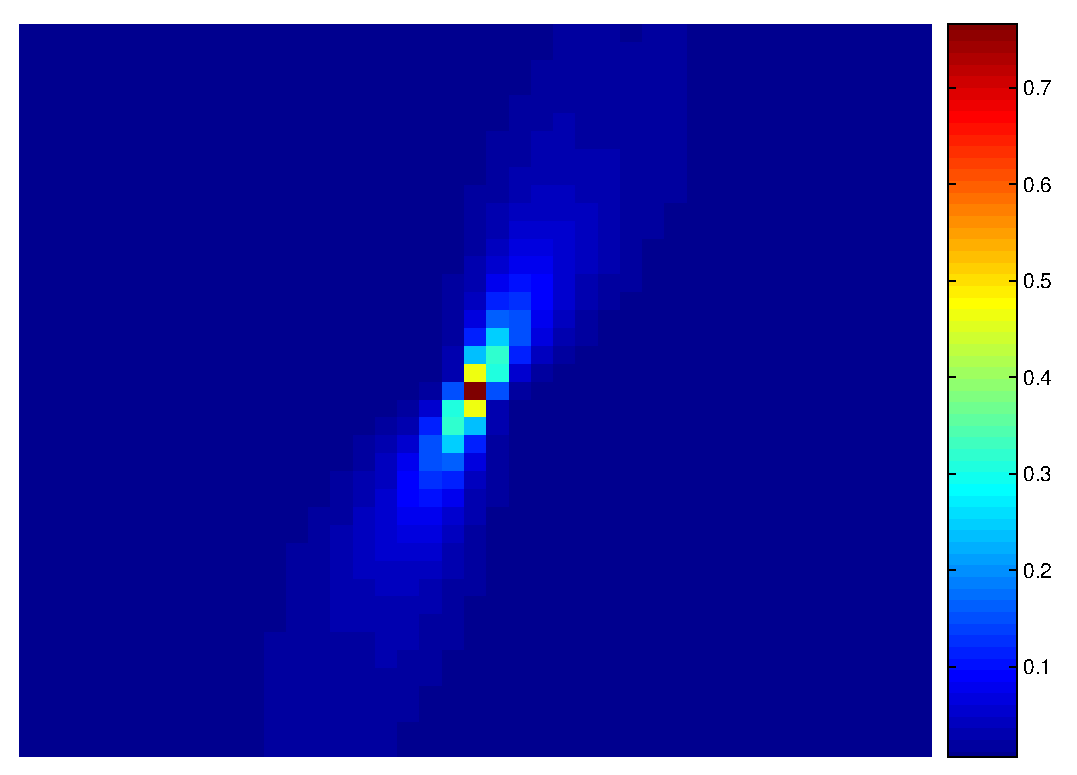
\includegraphics[width=0.8\linewidth]{./figs/af/or_l1l2_4}}
%	\end{center}
%  \caption{Difference between the two eigenvalues of the association field of figure \ref{fig:field2_e1_new}.}
%	\label{fig:field2_l1l2_new}
%\end{figure}


\begin{figure}[h]
	\begin{center}
		\begin{tabular}{cc}
			\fbox{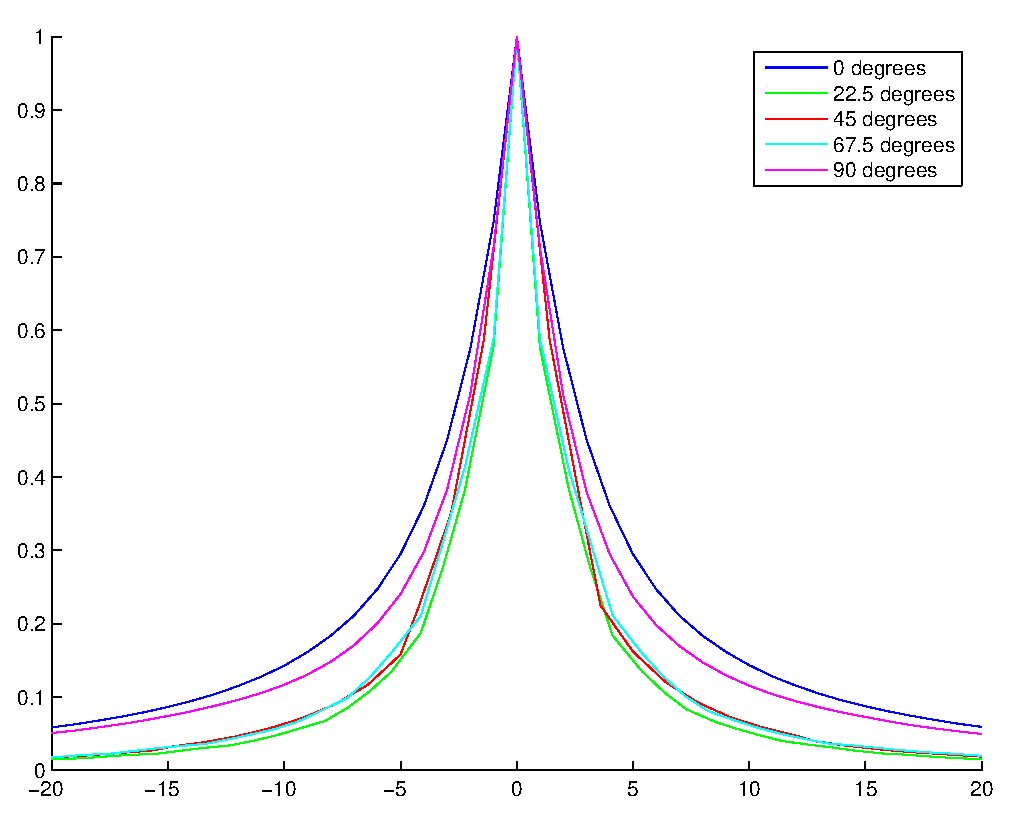
\includegraphics[height=0.4\linewidth]{./figs/af/confronto}} &
			\fbox{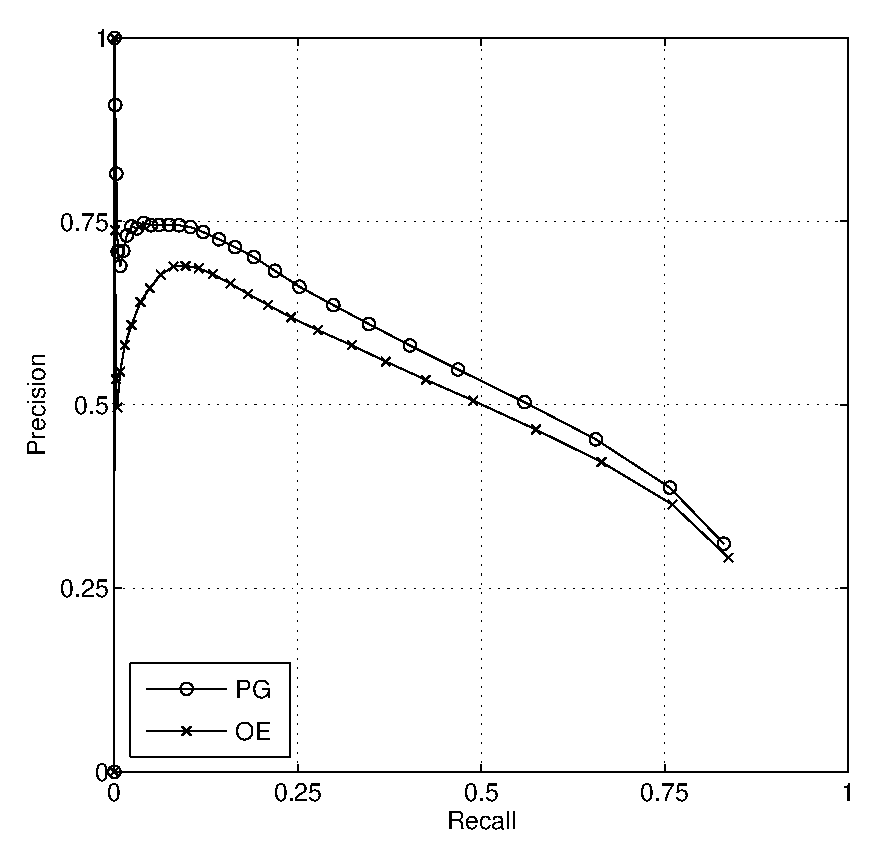
\includegraphics[height=0.4\linewidth]{./figs/af/pr_gray_011_012}} \\
			$(a)$ & $(b)$
		\end{tabular}
	  \caption{$(a)$ Comparison of the decay for the various orientations.
  	 On the y axis there are the first eigenvalues normalized to a
   	 maximum of $1$, on the x axis is the distance from the reference
     point along the main field direction.
     $(b)$ Comparison between tensor voting with learned fields (PG label) and the complex cell layer alone (OE label).}
	   \label{fig:conf}
	\end{center}
\end{figure}

%\begin{figure}[]
%	\begin{center}
%		\fbox{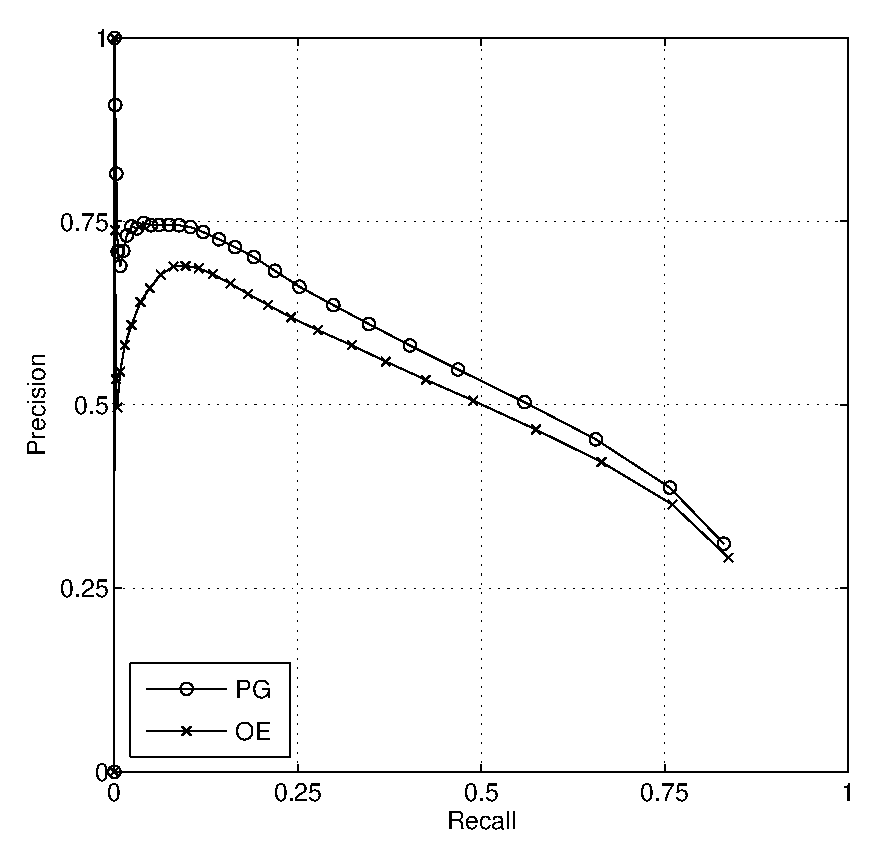
\includegraphics[width=0.8\linewidth]{./figs/af/pr_gray_011_012}}
%	\end{center}
%  \caption{Comparison between tensor voting with learned fields (PG label) and the complex cell layer alone (OE label).}
%	\label{fig:comp_oe_pg}
%\end{figure}

\begin{figure}[h]
	\begin{center}
		\begin{tabular}{cc}
			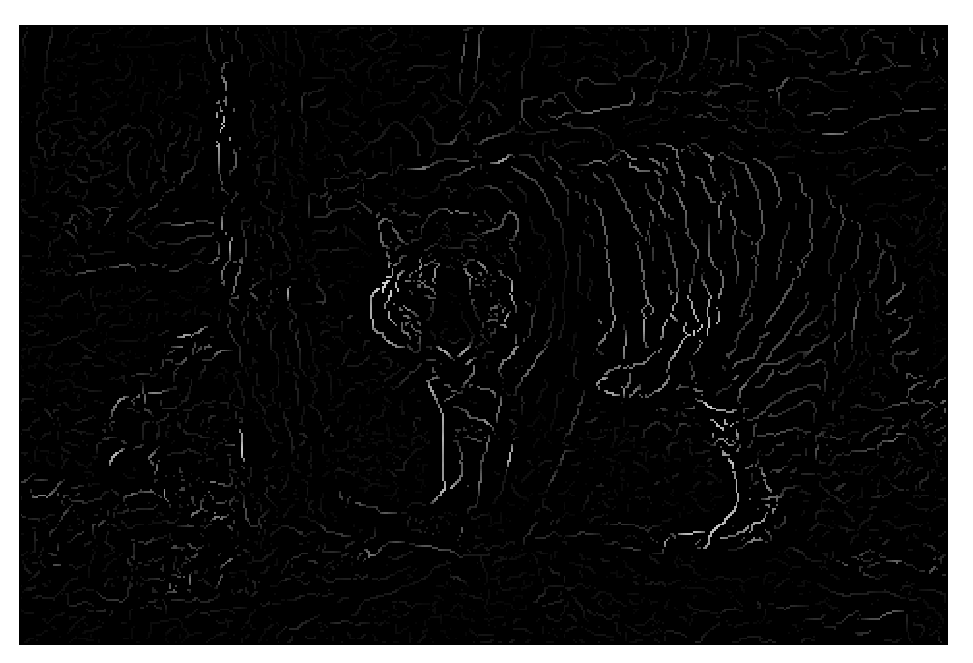
\includegraphics[width=0.4\linewidth]{./figs/af/im_oe} &
			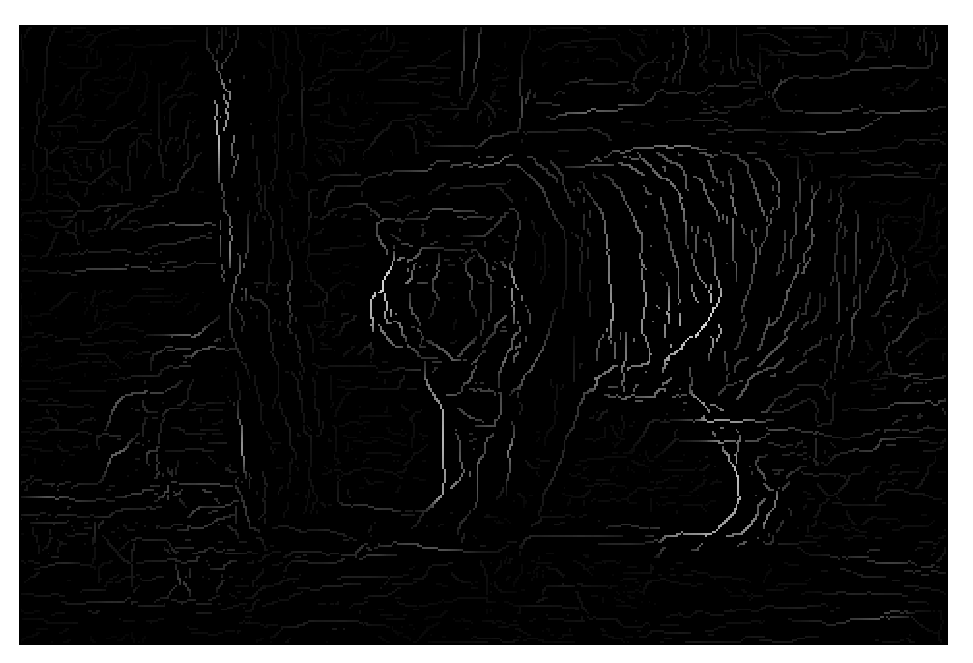
\includegraphics[width=0.4\linewidth]{./figs/af/im_pg} \\
			$(a)$ & $(b)$
		\end{tabular}
    \caption{$(a)$ Test image contours using the complex cell layer alone.
     $(b)$ Test image contours using tensor voting with the learned fields.
     Notice the differences with the $(a)$: the contours are
     linker together and the gaps are reduced. Especially on the contour of back of
     the tiger the differences are evident.}
	   \label{fig:im_oe_pg}
	\end{center}
\end{figure}


\section{Conclusion}
\label{sec:conclusion}

We have presented the general implementation of a visual
attention system employing both top-down and
bottom-up information. It runs in real time on a
standard Pentium class processor and it is used to
control the overt attention mechanism of a humanoid
robot. This eventually gives rise to a different sort of
problems compared to the more typical
implementations that only generate scan paths on static
images.
The algorithm divides the visual scene in color
blobs; each blob is assigned a bottom-up saliency value
depending on the contrast between its color and the
color of the surrounding area. The robot acquires
information about objects through active exploration
and uses it in the attention system as a top-down
primer to control the visual search of that object. The
model directs the attention on the proto-object's or
segmented object's center of mass (see Section \ref{sec:att_protoobj} and
Section \ref{sec:att_results}), similarly to the behavior observed in
humans. In fact it has been observed that the first
fixation to a simple shape that appears in the periphery
tends to land on its center of gravity \cite{MelcherK99}.
When the camera moves, a new blob will appear in
the image center. This active behavior simplifies the
segmentation and the recognition task since there will
always be a blob in the center that will be segmented
from the background.
A similar approach has been taken by Sun and
Fisher \cite{SunF03} but the main difference with this work is that
they have assumed that a hierarchical set of perceptual
groupings is provided to the attention system by some
other means and considered only covert attention.

In this sense we have tried to address this problem directly presenting a method to learn
precise association fields from natural images. A bio-inspired procedure
to get rid of the non-uniform distribution of orientations
is used, without the need of a tagged database of images \cite{ElderG02} nor
the use of motion \cite{Prodohl01}.
The learned fields were used in a computer model, using the tensor voting method,
and the results were compared using a database of human tagged images which helps
in providing clear numerical results.

Moreover the framework introduced is general enough
to work with other additional feature maps, extending the
watershed transform to additional dimensions in feature
space (e.g. local orientation) thus providing new ways
of both segmenting and recognizing objects.
As future work we want to integrate the associative fields
learnt from natural images to obtain better proto-objects.



%The main result from these studies is that these responses are not
%independent and they are highly correlated when they are arranged
%collinearly or on a common circle.



\bibliographystyle{splncs}
\bibliography{bibliografia}
\end{document}
